
\documentclass[a4paper,12pt]{article}
\usepackage[margin=2cm]{geometry}

% Pacchetti utili di base
\usepackage[utf8]{inputenc}   % codifica dei caratteri
\usepackage[T1]{fontenc}      % font encoding
\usepackage[italian]{babel}   % lingua italiana
\usepackage{graphicx}         % immagini
\usepackage{hyperref}         % link cliccabili
\usepackage{amsmath}          % align center
\usepackage{amssymb}    % simboli matematici extra (\mathbb, \nabla, ecc.)
\usepackage{amsfonts}   % font matematici aggiuntivi
\usepackage{amsthm}     % se vuoi definire teoremi, definizioni, ecc.
\usepackage{float}       % per immagini non float
\usepackage{tikz}        % per barra sopra
\usepackage{mathcomp} % per simbolo siile al dollaro con due barre
\usepackage{listings}
\usepackage{xcolor}
\usepackage{algorithm}
\usepackage{algpseudocode}

\lstset{
  basicstyle=\ttfamily\small,
  commentstyle=\color{gray},
  frame=single,
  breaklines=true
}

% Informazioni sul documento
\title{Ottimizzazione}
\author{Nicolò Giuliani}
\date{}


\begin{document}

\maketitle
\tableofcontents   % <-- genera automaticamente la pagina dell'indice
\newpage 
\section{Modelli di Problemi di Ottimizzazione}
\subsection{Intro}
\subsubsection{Preliminari}
\fcolorbox{blue!75!black}{blue!5!white}{
\parbox{\linewidth}{
\textbf{Definizione}: $z$ è \textbf{combinazione convessa} di $x,y$ se $\exists \lambda \in [0,1]$ t.c. $z=\lambda x + (1-\lambda)y$
\begin{figure}[H]
    \centering
    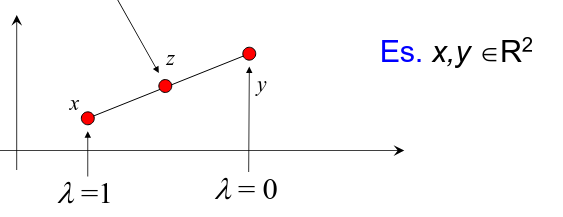
\includegraphics[width=0.5\textwidth]{img/z.png}
\end{figure}
}}\\
\vspace{1px}\\
\fcolorbox{blue!75!black}{blue!5!white}{
\parbox{\linewidth}{
\textbf{Definizione}: $z$ è \textbf{combinazione convessa di $K$ punti} $p_1, p_2, \dots, p_K \in \mathbb{R}^n$
\begin{align*}
  z =  \sum_{i=1,K}\lambda_i p_i \quad \text{ con } \lambda_i \geq 0\\
\end{align*}
e \begin{align*}
  \sum_{i=1,K} \lambda_i = 1
\end{align*}
\begin{figure}[H]
    \centering
    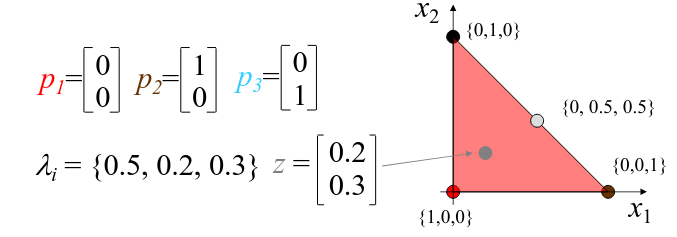
\includegraphics[width=0.5\textwidth]{img/z2.png}
\end{figure}
}}\\
\vspace{1px}\\
\fcolorbox{blue!75!black}{blue!5!white}{
\parbox{\linewidth}{
\textbf{Definizione} $F \subseteq \mathbb{R}^n$ è un \textbf{insieme convesso} se 
\begin{align*}
  \forall x,y \in F \text{ e } \forall \lambda \in [0,1] \\
  z = \lambda x + (1-\lambda)y \in F
\end{align*}
\begin{figure}[H]
    \centering
    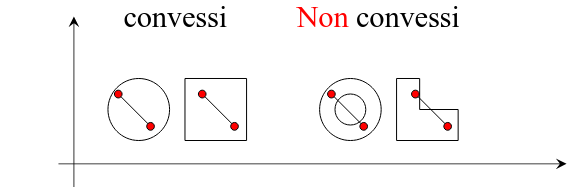
\includegraphics[width=0.5\textwidth]{img/convessi.png}
\end{figure}
}}\\
\vspace{1px}\\
Proprietà degli insiemi convessi:
\begin{itemize}
  \item $\mathbb{R}^n$ è convesso
  \item Se abbiamo $F_i$ convessi allora $F = \bigcap F_i$ è convesso
\end{itemize}
\begin{figure}[H]
    \centering
    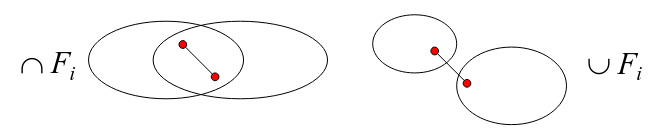
\includegraphics[width=0.5\textwidth]{img/convesso_intersezione.png}
\end{figure}
\fcolorbox{blue!75!black}{blue!5!white}{
\parbox{\linewidth}{
\textbf{Definizione}: $z$ è \textbf{vertice} di un insieme convesso $F$ se e solo se non è combinazione convessa di altri punti di $F$
}}\\
\vspace{1px}\\
\fcolorbox{blue!75!black}{blue!5!white}{
\parbox{\linewidth}{
\textbf{Definizione}: dato un insieme di punti $P=\{p_1, \dots, p_K\} \subset \mathbb{R}^n$ si dice \textbf{chiusura convessa} di $P$ (\textit{conv(P)}) il più piccolo insieme che contiene $P$.
\begin{figure}[H]
    \centering
    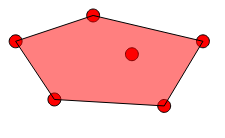
\includegraphics[width=0.3\textwidth]{img/p.png}
\end{figure}
}}\\
\vspace{1px}\\
\fcolorbox{blue!75!black}{blue!5!white}{
\parbox{\linewidth}{
\textbf{Definizione}: Dato $F \subseteq \mathbb{R}^n$ convesso, allora 
\begin{align*}
  \phi \, : \, F \to R
\end{align*}
è convessa se:
\begin{align*}
  \forall x,y \in F, \, \forall \lambda \in [0,1]1
\end{align*}
si ha allora:
\begin{align*}
  \phi (\lambda x + (1 - \lambda)y) \leq \lambda \phi (x) + (1 - \lambda) \phi (x)
\end{align*}
\begin{figure}[H]
    \centering
    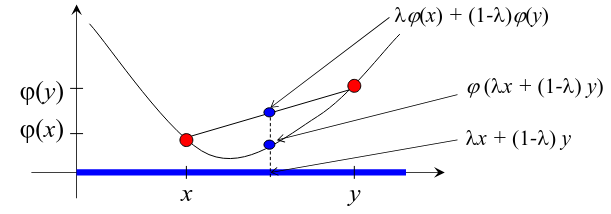
\includegraphics[width=0.51\textwidth]{img/funzione.png}
\end{figure}
}}\\
\vspace{1px}\\
\subsubsection{Problemi di ottimizzazione}
Un prolema di ottimizzazione cerca la risposta che dipende da parametri e variabili. Un problema $P$ viene descritto dai suoi parametri, variabili e i loro legami; e la descrizione delle soluzioni che devono avere. \\
Un'\textbf{istanza} del problema $P$ si ottiene specificando valori concreti per tutti i parametri (NON VARIABILI!)
\begin{figure}[H]
    \centering
    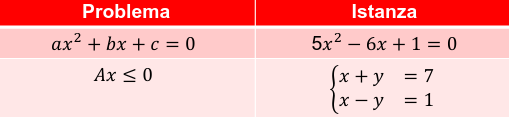
\includegraphics[width=0.51\textwidth]{img/problema.png}
\end{figure}
Possiamo dire che
\begin{itemize}
  \item $x = (x_1, \dots, x_n) \in F'$ vettore di \textbf{variabili decisionali}
  \item $F \subseteq F'$ insieme \textbf{soluzioni ammissibili}
  \item $c \, : \, F \to \mathbb{R}$ funzione \textbf{costo}
\end{itemize}
Per esempio vogliamo trovare il minimo con
\begin{align*}
  (P) \quad \min{c(x) : x \in F}
\end{align*}
ovvero trovare $x^* \in F$ (ottimo globale) tale che
\begin{align*}
  z(P) = c(x^*) \leq c(x) \, \forall x \in F
\end{align*}
\begin{figure}[H]
    \centering
    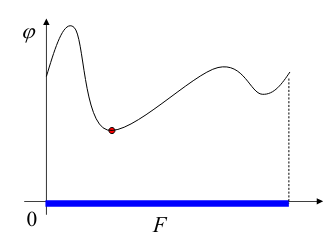
\includegraphics[width=0.3\textwidth]{img/min.png}
\end{figure}
I problemi di ottimizzazione posso essere sia di minimizzazione che massimizzazione.\\
Dato $(P) \quad \min{c(x) : x \in F}$, il problema $(P') \quad -\max{-c(x) : x \in F}$ è equivalente a $(P)$. Ossia $z(P)=z(P')$, i due problemi hanno lo stesso insieme di soluzioni ottime.
\begin{figure}[H]
    \centering
    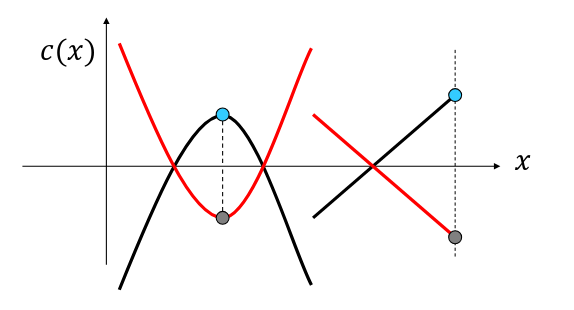
\includegraphics[width=0.4\textwidth]{img/max.png}
\end{figure}
\paragraph{Regione ammisibile}
La regione ammissibile di $F$ può essere definita come
\begin{itemize}
  \item esplicitamente: specificando le proprietà di $x \in F$
  \item implicitamente: attraverso equazioni e disequazioni
\end{itemize}
\begin{figure}[H]
    \centering
    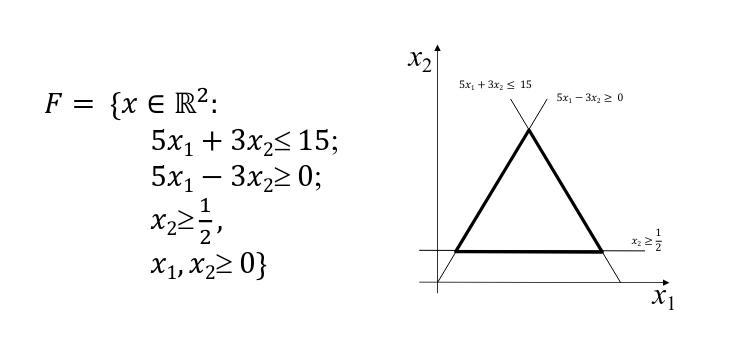
\includegraphics[width=0.5\textwidth]{img/regione.png}
\end{figure}
 Vedremo come sia più conveniente avere solo una tipologia di forma (solo disequazioni/equazioni, ecc). Dato un modello in forma generale possiamo costruire un nuovo modello con la forma desiderata. Per esempio
 \begin{align*}
    \min\{c(x) \, : \, x \in F\} = - \max\{-c(x) \, : \, x \in F\}
 \end{align*}
\begin{itemize}
  \item Da disequazione a equazione:
  \begin{itemize}
    \item  $x_1 \leq d_1 \quad \to x_1 + x_s = d_1$ con $x_s$ variabile \textbf{slack}
    \item $x_1 \geq d_1 \quad \to x_1 - x_s = d_1$ con $x_s$ variabile \textbf{surplus}
  \end{itemize}  
  \item Da equazione a disequazione
  \begin{align*}
      a_j^T x = d_i \to \begin{cases}
        a_j^T x \geq d_j \\
        -a_j^T x \geq -d_j
      \end{cases}
  \end{align*}
\end{itemize}
Le trasformazioni possono aumentare i vincoli o le variabili del modello rispetto a quello originale.\\
\paragraph{Segno delle variabili} Generalmente le variabili sono vincolate ($x_j \geq 0$ o $x_j \leq 0$), nel caso non avessimo i vincoli ci si può sempre ricondurre ad un modello con variabili tutte $\geq 0$
\begin{align*}
  x_j \leq 0 \quad \to y_i = -x_j \geq 0
\end{align*}
\paragraph{Soluzioni}
Abbia quattro casi possibili:
\begin{itemize}
  \item Problema impossibile: ($F = \emptyset$), allora si assume $z(P) = + \infty$
  \item Problema inferiormente (superiormente) illimitato: scelto un numero $M$ abbiamo una soluzione $x \in F$ t.c. $c(x) \leq M$ (o $\geq M$)
  \item Il problema ha valore ottimo finito $- \infty < z(P) < \infty$ ma non ha soluzione ottima (non esiste $x \in F$ t.c. $c(x)=z(P)$
  \item Il problema ha valore ottimo finito ed ammette soluzione ottima
\end{itemize}
\paragraph{Minimi Locali e Globali} Non è detto che esista $x^*$ ($F = \emptyset$) o che sia unica. Possono esistere ottimi (minimi) locali e globali
\begin{figure}[H]
    \centering
    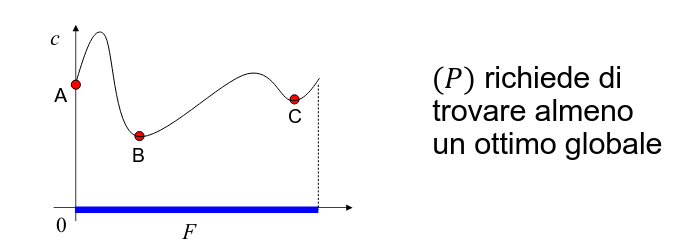
\includegraphics[width=0.5\textwidth]{img/minimo.png}
\end{figure}
La risoluzione di un problema di ottimizzazione richiede l'impiego di un metodo di calcolo (numerico e iterativo) codificato mediante un algoritmo.
\begin{itemize}
  \item Algoritmo \textbf{esatto} per $P$: dato un'istanza di $P$ fornisce in output la soluzione ottima $x^*$ di $P$ (se esiste)
  \item Algortimo \textbf{euristico} per $P$: determina una qualsiasi soluzione $x \in F$ attraverso una approssimazione (minimo/massimo)
  \begin{itemize}
    \item Dato $\epsilon$-approssimazione allora $x$ è approssimato se $c(x) \leq \epsilon$.
    \begin{align*}
    \text{Errore assoluto}: \epsilon_P = | c(x) - z(P) |\\
    \text{Errore relativo}: R_P = \frac{\epsilon_P}{|z(P)|} = \frac{| c(x) - z(P) |}{|z(P)|}
    \end{align*}
  \end{itemize}
\end{itemize}
Alcune volte anche calcolare l'errore diventa un problema se $z(P)$ non è noto. Allora risolviamo un nuovo problema approssimando quello originale.\\
Dato $P$ definiamo \textbf{rilassamento} di $P$ un problema del tipo
\begin{align*}
  \overline{P}= \min\{\overline{c}(x)\ \, : \, x \in \overline{F}\}
\end{align*}
t.c.
\begin{itemize}
  \item $z(\overline{P}) \leq z(P)$
  \item $F \subseteq \overline{F}$ e $\forall x \in \overline{F}, \, \overline{c}(x) \leq c(x)$
  \item Se la soluzione ottima $\overline{x}^*$ di $\overline{P}$ soddisfa $\overline{x}^* \in F$ e $\overline{c}(\overline{x}^*) = c(\overline{x}^*)$ allora è ottima anche per $P$
\end{itemize}
Ovviamento gli algoritmi numerici non hanno una visione completa di $c$ e $F$ ma valuta $c(x)$ solo per un intervallo limitato di $x \in F$. Generalmente gli algoritmi di ottimizzazione sono iterativi, la soluzione converge verso una soluzione ottima (locale) con iterazioni molto alte o quando si raggiunge una approssimazione desiderata.\\
\fcolorbox{blue!75!black}{blue!5!white}{
\parbox{\linewidth}{
\textbf{Definizione}: $y \in F$ è \textbf{ottimo locale} se $\exists$ un interno $N \subseteq F$ tale che $c(y) \leq c(x) \, \forall x \in N$
\begin{figure}[H]
    \centering
    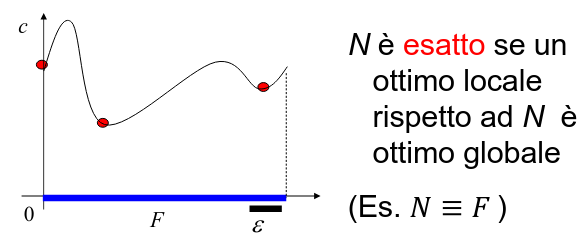
\includegraphics[width=0.5\textwidth]{img/ott_loc.png}
\end{figure}
}}\\
\vspace{1px}\\
\fcolorbox{blue!75!black}{blue!5!white}{
\parbox{\linewidth}{
\textbf{Teorema}: Dato $P(F,c)$ con $F \subseteq \mathbb{R}^n$ convesso e $c$ convessa, l'intorno euclideo $N_\epsilon(y) = \{x \in F \, : \, \|y-x \| \leq \epsilon\}$ è \textbf{esatto} $\forall \epsilon > 0$.\\
Ottimo locale $\equiv$ ottimo globale
\begin{figure}[H]
    \centering
    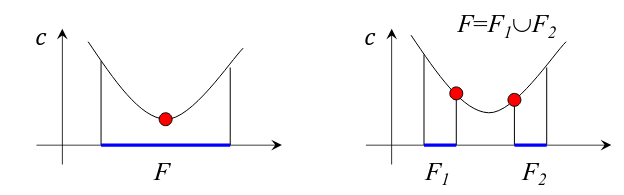
\includegraphics[width=0.5\textwidth]{img/eu.png}
\end{figure}
}}\\
\vspace{1px}\\

Dimostrazione: OC2026-2-Intro\_Ottimizzazione - Ver.2.0.pdf, pagina 40.
\vspace{1px}\\
\subsection{Modelli}
Definito il problema dobbiamo classificarlo su un certo tipo. Attraverso un modello favoriamo l'astrazione e similitudini. Ci occuperemo di programmazione lineare: \\
Un problema di programmazione lineare (PL, LP) è un problema di ottimizzazione definito da
\begin{itemize}
  \item numero finito di variabili decisionali $n \in \mathbb{N}$: $x = (x_1, \dots, x_n) \in \mathbb{R}^n$
  \item funzione obbiettivo $f \, : \, \mathbb{R}^n \to \mathbb{R}$ nella forma $f(x)=c(x)$
  \item insieme $m$ di vincoli lineari in una delle seguenti forme $ax=b, \, ax \leq b, \, ax \geq b$ con $a \in \mathbb{R}^n , b \in \mathbb{R}$
\end{itemize}
Alcune volte dobbiamo assumere $z \in Z^n$ vettore delle soluzioni (di numeri interi). Allora siamo in caso di programmazione lineare intera (PLI, ILP) o programmazione lineare mista (PLM, MILP) se solo una parte delle variabili sono intere.
\begin{figure}[H]
    \centering
    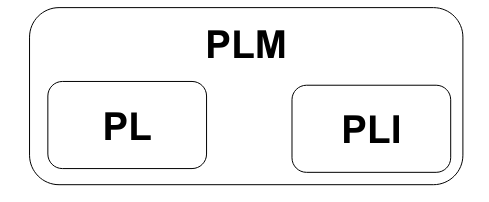
\includegraphics[width=0.5\textwidth]{img/plm.png}
\end{figure}
Possiamo definire un problema PL nella seguente forma
\begin{align*}
  \min \{cx | Ax \leq b \}
\end{align*}
con $A \in \mathbb{R}^{m \times n}, \, b \in \mathbb{R}^m$. \\
\textbf{Variabili booleane}: condizioni binarie (0,1), spesso vengono usate come variabili ausiliarie per che stabiliscono il verificarsi o meno di condizioni specifiche.
\subsubsection{Problema dello zaino}
Dato uno zaino di capacità $b$ e un insieme $E=\{1,2,\dots,n\}$ di $n$ oggetti caraterizzato da peso $a_i$ e profitto $c_i$. Determinare il sottoinsieme $S \subseteq E$ t.c. profitto massimo e peso totale inferiore a $b$.
\begin{align*}
  F = \{S \subseteq E \, : \, \sum_{i \in S} a_j \leq b\}\\
  c(S) = \sum_{i \in S} c_j
\end{align*}
Le soluzioni sono tutti i sottoinsiemi di $E$ t.c $2^{|E|}=2^n$. \\
La soluzione ottimale è
\begin{align*}
  S^* = \min\{c(S) \, : \, S \in F\}
\end{align*}
Selezione:
\begin{align*}
\forall i=1,\dots,n \quad x_i = \begin{cases}
  1 \text{ se $i$ selezionato ($\in S^*$)}\\
  0 \text{ altrimenti}
\end{cases}\\
\max c(x) = \sum_{i=1}^n c_i x_i
\end{align*}
KP: 
\begin{align*}
  \sum_{i=1}^n a_i x_i \leq b \quad x_i \in {0,1}
\end{align*}
\subsection*{Min-cost Spanning Tre}
Dato un grafo non orientato $G=(N,A)$, con $|N|=n, \, |A|=m$ e $\forall a \in A \, c_a \geq 0$. Vogliamo cerchare il grafo parziale $G'=(N,A')$ connesso e aciclico di costo minimo
\begin{align*}
  F = \{T \subseteq A \, : \, (N,T) \text{ è uno $ST$ di $G$}\}\\
  c(T) = \sum_{a \in A} c_a
\end{align*}
La soluzione ottima è $T^* = \min\{c(T) \, : \, T \in F\}$.\\
Selezione:
\begin{align*}
  \forall a \in A, \quad x_a = \begin{cases}
  1 \text{ se $a$ selezionato ($\in T^*$)} \\
  0 \text{ altrimenti}
  \end{cases}
\end{align*}
\subsubsection{Problema MST}
\begin{align*}
  \forall a \in A, \quad x_a = \begin{cases}
  1 \text{ se $a$ selezionato ($\in T^*$)}\\
  0 \text{ altrimenti}
  \end{cases}\\
  \min c(x) = \sum_{a \in A} c_a x_a
\end{align*}
MST:
\begin{align*}
  \sum_{a \in A(N', N'')} x_a \geq 1 \quad \forall (N', N'') \quad x_a \in \{0,1\} \quad a \in A
\end{align*}
\subsubsection{Problema TSP}
Traveling salesman problem
\begin{align*}
  F = \{P \subseteq A \, : \,(N,P) \text{ è ciclo Hamiltoniano di $G$}\}\\
  c(P) = \sum_{(i,j) \in P} c_{i,j}
\end{align*}
Dovendo visitare ogni nodo una sola volta $P$ dovrà contenere esattamente due archi incidenti in ciascuna città : $\sum_{j:(i,j) \in A} = 2$
Soluzione ottima:
\begin{align*}
  P^* = \min\{c(P) \, : \, P \in F\}
\end{align*}
Selezione:
\begin{align*}
\forall (i,j) \in A, \quad x_{ij} = \begin{cases}
  1 \text{ se $(i,j)$ selezionato ($\in P^*$)}\\
  0 \text{ altrimenti}
\end{cases}\\
\min c(x) = \sum_{(i,j) \in A} c_{ij}x_{ij}
\end{align*}
TSP:
\begin{align*}
  \sum_{(i,j) \in A(N', N'')} x_{ij} \geq 1 \quad \forall (N',N'') \quad x_{ij} \in {0,1} \quad (i,j) \in A
\end{align*}
Notiamo come MST è un rilassamento di TSP!
\subsection*{Relazioni logiche tra variabili} 
Le relazioni logiche tra operatori hanno natura logica. Possiamo modificare le relazioni logiche attraverso vincoli lineari.
\begin{itemize}
  \item \textbf{Negazione}: $y = \neg x \Rightarrow y = 1 -x$
  \item \textbf{Implicazione}: $x \to y \Rightarrow y \geq x$ (se $x=0$ $y$ è libera)
  \item \textbf{Intersezione (AND)}: $z = (x \land y) \Rightarrow \begin{cases}
    z \leq x \\
    z \leq y \\
    z \geq x + y-1
  \end{cases}$
   \item \textbf{Unione (OR)}: $z = (x \lor y) \Rightarrow \begin{cases}
    z \geq x \\
    z \geq y \\
    z \leq x + y
  \end{cases}$
\end{itemize}
\paragraph{Vincoli di assegnamento}
Spesso dobbiamo modellare associazioni tra entità del problema.
\begin{align*}
  \forall (i,j) \quad x_{ij}= \begin{cases}
    1 \text{ se oggetto $i$ assenato a lugo $j$}\\
    0 \text{ altrimenti}
  \end{cases}
\end{align*}
\begin{itemize}
  \item Semi-assegnamento: ogni oggetto può essere assegnato ad 1 solo luogo
  \begin{align*}
      \sum_{j=1}^m x_{ij}=1 \quad i=1,\dots,n
  \end{align*}
  \item Assegnamento completo: ogni oggetto può essere assegnato ad 1 solo luogo, ad ogni luogo un solo oggetto
\end{itemize}
\begin{figure}[H]
    \centering
    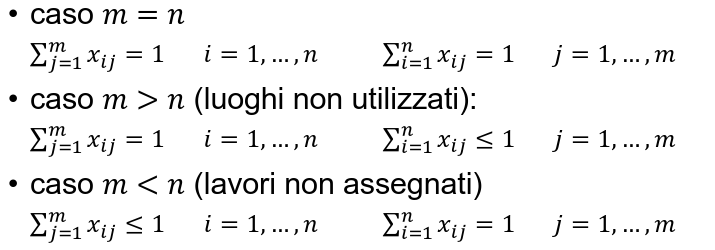
\includegraphics[width=0.5\textwidth]{img/luogo.png}
\end{figure}
\subsection*{Ordinamento di lavori su macchine}
Dati $n$ lavori, il loro tempo di lavoro $d_i$ e $m$ macchine identiche. Dobbiamo assegnare i lavori alle macchine senza sovrapposizione e minimizzando il numero di macchine usate.
\subsubsection{Problema Min Cardinality Machine Scheduling}
Due lavori possono essere lavorati sulla stessa macchina se gli intervalli di lavorazione sono disgiunti. Se gli intervalli di lavorazione sono sovrapposti due lavori non possono essere eseguiti sulla stessa macchina.
\begin{figure}[H]
    \centering
    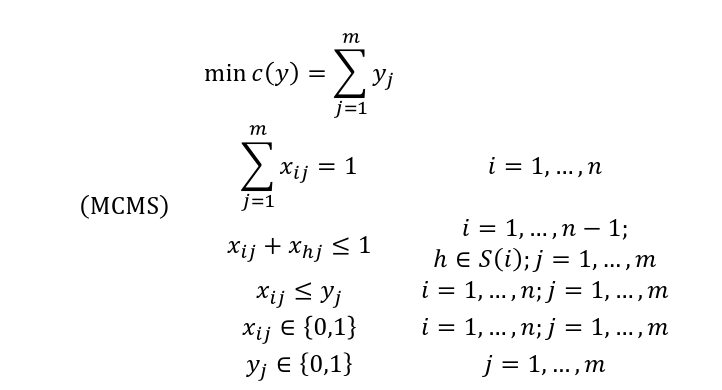
\includegraphics[width=0.7\textwidth]{img/macchine.png}
\end{figure}
\subsubsection{Selezione di sottoinsiemi}
$N$ insieme di elementi, $F={F_1,\dots,F_n}$ famiglia di suoi sottoinsiemi. Dobbiamo trovare un insieme di sottoinsiem $D$ di costo minimo che soddisfi i vincoli.
\subsubsection{Set Covering Problem}
$D$ richiede di selezionare un sottoinsieme di $F_j$.
\begin{align*}
  x_j = \begin{cases}
    1 \text{ se $j \in D$}\\
    0 \text{ altrimenti}
  \end{cases} \quad j=1,\dots,m 
\end{align*}
Funzione obbiettivo:
\begin{align*}
  \min \sum_{j=1}^m c_j x_j
\end{align*}
\subsubsection*{Set Covering Problem}
ogni elemento $i \in N$ deve essere in almeno un sottoinsieme di $D$.
\begin{align*}
    \sum_{j=1}^m a_{ij}x_j \geq 1 \quad i = 1,\dots, n \\
    \min c(x)= \sum_{j=1}^m c_j x_j
\end{align*}
SCP:
\begin{align*}
  \sum_{j=1}^m a_{ij}x_j \geq 1 \quad i = 1,\dots,n\\
  x_j \in \{0,1\} \quad j=1,\dots,m
\end{align*}
\subsubsection*{Set Partitioning Problem}
ogni elemento $i \in N$ deve essere esattamente in un sottoinsieme di $D$.
\begin{align*}
    \sum_{j=1}^m a_{ij}x_j \geq 1 \quad i = 1,\dots, n \\
      \min c(x)= \sum_{j=1}^m c_j x_j
\end{align*}
SPP:
\begin{align*}
      \sum_{j=1}^m a_{ij}x_j = 1 \quad i = 1,\dots, n \\
      x_j \in \{0,1\} \quad j=1,\dots,m
\end{align*}
\subsubsection*{Set Packing Problem}
ogni elemento $i \in N$ deve essere al più in un sottoinsieme di $D$.
\begin{align*}
  \sum_{j=1}^m a_{ij}x_j \leq 1 \quad i=1,\dots,n
\end{align*}
\begin{itemize}
  \item problema di min: $D = \emptyset$
  \item prolema di max:
  \begin{align*}
    \max c(x) = \sum_j=1^m c_j x_j
  \end{align*} 
  SPkP
  \begin{align*}
      \sum_{j=1}^m a_{ij}x_j \leq 1 \quad i=1,\dots,n\\
      x_j \in \{0,1\} \quad j=1,\dots,m
  \end{align*}
\end{itemize}
\subsection*{Variabili a valori discreti}
Spesso le variabili sono vincolate ad assumere valori in un insieme che è $\{0,1\}, N, [\dots]$. Per esempio $x$ deve appartenere ad un insieme $\{v_1,\dots,v_k\}$ di valori reali.\\
Introduciamo $k$ varbiabili binarie $y_i \in \{0,1\}$ t.c.
\begin{align*}
    \sum_{i=1}^ky_i = 1 \quad x= \sum_{i=1}^k v_i y_i
\end{align*}
\subsubsection{Progetto di reti}
I collegamenti della rete sono descritti da un grafo orientato $G(V,A)$ con $b_i$ come quantità massima per arco. \\
Per ogni nodo della rete il flusso portato dagli archi uscenti deve essere = al flusso entrante più la quantità prodotta nel nodo.
\subsubsection*{Minima quantità positiva}
Quando $x$ rappresenta un livello di produzione lo possiamo definire $\{0\} \cup [l,u]$. (0 rappresenta l'assenza di produzione). Introduciamo $y \in \{0,1\}$ che ci indica la presenza di produzione
\begin{align*}
    ly \leq x \quad x \leq uy
\end{align*}
\subsubsection{Costo fisso di produzione}
Funzione con carico fisso, problema di mix di produzione. Se non produciamo prodotto ($x_j = 0$) allora non abbiamo costi, se produciamo ($x_j > 0$) allora abbiamo un costo fisso $F_j$ più un costo variabile $p_j x_j$. 
\begin{figure}[H]
    \centering
    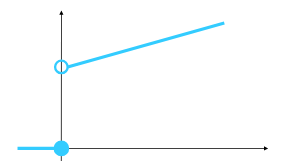
\includegraphics[width=0.5\textwidth]{img/costofisso.png}
\end{figure}
\begin{align*}
  y_j = \begin{cases}
    1 \text{ se $x_j > 0$}\\
    0 \text{ se $x_j = 0$}
  \end{cases}
\end{align*}
\begin{align*}
  & \min \sum_{j=1}^n F_j y_j + p_j x_j \\
  & Ax \geq b \\
  & x \geq 0 \\
  & y \in \{0,1\}^n
\end{align*}
Validita' del vincolo:
\begin{itemize}
  \item se $x_j > 0$ allora $y_j = 1$ e il vincolo $x_j \leq + \infty$
  \item se $x_j = 0$ allora $y_j = 0$ o $y_j = 1$
\end{itemize}
oppure
\begin{itemize}
  \item se $y_j = 0$ allora $x_j = 0$ 
  \item se $y_j = 1$ allora $x_j \geq 0 \,(\leq  + \infty)$
\end{itemize}
Quindi cerchiamo
\begin{align*}
  & \min \sum_{j=1}^n F_j y_j + p_j x_j \\
  & Ax \geq b \\
  & x_j \leq My_j \\
  & x_j \geq 0 \\
  & y_j \in \{0,1\}
\end{align*}
\subsubsection{Ordinamento di lavori su macchine}
Variante di MCMS, dati $n$ lavori, $m$ macchine identiche. Assegnare i lavori alle macchine senza sovrapposizione e minimizzando il tempo massimo di completamento dei lavori sulle macchine.
\begin{align*}
  \forall (i,j) \quad x_{ij} = \begin{cases}
    1 \text{ se lavoro $i$ assegnato a macchina $j$}\\
    0 \text{ altrimenti}
  \end{cases} \quad i=1,\dots,n \quad j=1,\dots,m
\end{align*}
Ogni lavoro deve essere assegnato ad una macchina
\begin{align*}
  \sum_{j=1}^m x_{ij} = 1 \quad i=1,\dots,n
\end{align*}
Il tempo di completamento di una macchina $j$ è la somma dei tempi di lavorazione dei lavori assegnati a essa:
\begin{align*}
  t_j = \sum_{i=1}^n d_i x_{ij} \quad j=1,\dots,m
\end{align*}
Il tempo massimo di completamento è $t_{max} = \max\{t_j \, | \, j=1,\dots,m\}$, che puo' essere definito da $m$ vincoli lineari:
\begin{align*}
  t_j \geq \sum_{i=1}^n d_i x_{ij} \quad j=1,\dots,m
\end{align*}
\subsubsection{Min Makespan Machine Scheduling}
Anche noto come $P || C_{\max}$.
\begin{align*}
  \min_t \sum_{j=1}^m x_{ij} \\
\end{align*}
MMMS:
\begin{align*}
  & \sum_{j=1}^m x_{ij} \leq t\\
  & x_{ij} \in \{0,1\} \quad i=1,\dots,n \quad j=1,\dots,m
\end{align*}
\subsubsection*{Valore Assoluto} 
Dobbiamo rappresentare $|g(x)|$.\\
\textbf{Vincoli}: $|g(x)| \leq b$ puo' essere espresso dalla coppia di vincoli $g(x) \leq b$ e $-g(x) \leq b$.\\
\textbf{Funzione obbiettivo}: $z = \min |g(x)|$ puo' essere calcolato risolvendo separatamente $z' = \max \{f(x) \, | \, x \in F\}$ e $z'' = \max\{f(x) \, | \, x \in F\}$, e definiamo $z = \max\{z', z''\}$.
\subsubsection*{Funzioni lineari a tratti}
Come nel carico fisso si possono usare variabili binarie per rappresentare funzioni lineari a tratti.\\
\begin{align*}
  y_1 = \begin{cases}
    1 \text{ se $x \in [a_1, a_2]$}\\
    0 \text{ altrimenti}
  \end{cases} \quad y_2 = \begin{cases}
    1 \text{ se $x \in (a_2, a_3]$}\\
    0 \text{ altrimenti}
    \end{cases}
\end{align*}
Poiche' $x$ deve appartenewre ad un solo intervallo, allora $y_1 + y_2 = 1$.\\
Introduciamo anche 2 variabili usiliare quantitative:
\begin{align*}
  z_1 = \begin{cases}
    x-a_1 \text{ se $x \in [a_1, a_2]$}\\
    0 \text{ altrimenti}
  \end{cases} \quad z_2 = \begin{cases}
    x-a_2 \text{ se $x \in (a_2, a_3]$}\\
    0 \text{ altrimenti}
  \end{cases}
\end{align*}
Le variabili ausiliare sono completamente definite dai vincoli
\begin{align*}
  & 0 \leq z_1 \leq (a_2 - a_1) y_1 \\
  & 0 \leq z_2 \leq (a_3 - a_2) y_2 \\
  & y_1 + y_2 = 1 \\
  & y_1, y_2 \in \{0,1\}
\end{align*}
\subsubsection*{Funzioni convesse}
Una funzione $f$ lineare ad $n$ tratti e' convessa se e' continua e la derivata non crescente.\\
\subsubsection{min Funzioni convesse}
\begin{align*}
  \min b_1 + c_1 a_1 + \sum_{i=1}^n z_i\\
  0 \leq z_i \leq a_{i+1} - a_i \quad i=1,\dots,n-1\\
\end{align*}
Se il valore ottimo e' $\bar{x}$ si avra':
\begin{align*}
  z_i = a_{i+1} - a_i \quad i=1,\dots,h\\
  z_h = \bar{x} - a_h \quad i=h\\
  z_i = 0 \quad i=h+1,\dots,n
\end{align*}
Analogamente vale per le $\max$ funzioni concave.
\subsubsection{Modello PLI}
Funzioni a tratti
\begin{figure}[H]
    \centering
    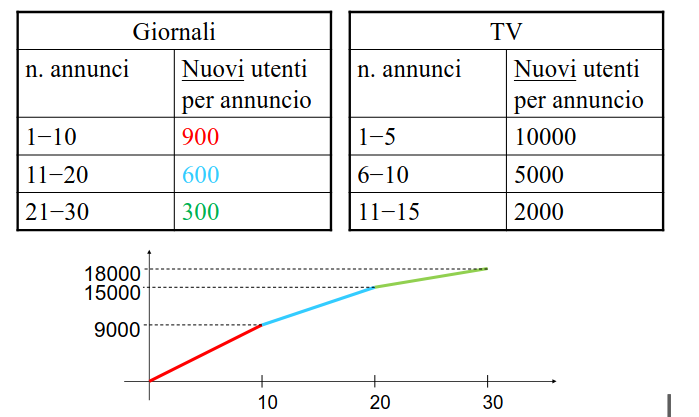
\includegraphics[width=0.5\textwidth]{img/tratti.png}
\end{figure}
Si possono utilizzare variabili binarie per rappresentare funzioni a tratti, per indicare se le variabili decisionali sono nella prima, seconda, terza fascia. Vincoli di tipo logico come per il costto fisso.\\
\begin{align*}
  \max 900G_1 + 600G_2 + 300G_3 + 10000T_1 + 5000T_2 + 2000T_3\\
  G_1 + G_2 + G_3 + 10T_1 + 10T_2 + 10T_3 \leq 150\\
  G_1, G_2, G_3 \leq 10\\
  T_1, T_2, T_3 \leq 5\\
  G_1, G_2, G_3, T_1, T_2, T_3 > 0 \text{ INTERE}
\end{align*}
\subsubsection{Altri modelli PLI}
\subsubsection*{Variante KP: KP-bounded}
Il generico oggeto $i$ e' disponibile in $p_i$ esemplari. Puo' essere scelto $p_i$ volte
\begin{align*}
  \forall i=1, \dots, n \, x_i \geq 0 \text{ intera} = \text{ n. di copie $i$ scelte}\\
  \max c(x) = \sum_{i=1}^n c_i x_i\\
\end{align*}
KP-b:
\begin{align*}
  \sum_{i=1}^n a_i x_i \leq b\\
  0 \leq x_i \leq p_i \text{ interi } \quad i=1,\dots,n 
\end{align*}
\subsubsection*{Variante KP: Subset-sum Problem}
Il generico oggetto $i$ ha profitto $c_i$ e peso $a_i = c_i$. Dato un insieme di $n$ numeri selezionare un sottoinsieme di numeri di somma massima e non eccedente a $b$. (Taglio di barre e minimizzazione scarto)
\begin{align*}
  \forall i=1,\dots,n \quad x_i = \begin{cases}
    1 \text{ se $i$ selezionato ($\in S^*$)}\\
    0 \text{ altrimenti}
  \end{cases}\\
  \max c(x) = \sum_{i=1}^n c_i x
\end{align*}\\
SSP:
\begin{align*}
  \sum_{i=1}^n c_i x_i \leq b\\
  x_i \in \{0,1\} \quad i=1,\dots,n
\end{align*}
\subsubsection*{Problema KP multiplo (MKP)}
\subsubsection*{Modello MKP}
$n$ oggetti, $c_i$ profitto, $a_{ij}$ peso su risorsa $j$. $m$ continitori di capacita' $b_j$. Un oggetto puo' andare al piu' in un contenitore, ogni contenitore puo' contenere piu' oggetti. \\
Impaccare nei contenitori un sottoinsieme di oggetti avente massimo profitto in modo che la somma dei pesi degli oggetti inseriti in ogni contenitore non superi la corrispondente capacità $b_i$.
\begin{align*}
  \forall i,j \quad x_{ij} = \begin{cases}
    1 \text{ se $i$ inserito nel contenitore $j$}\\
    0 \text{ altrimenti}
  \end{cases}\\
  \max c(x) = \sum_{i=1}^n \sum_{j=1}^m c_i x_{ij}\\
  \sum_{j=1}^m x_{ij} \leq 1 \quad i=1,\dots,n
\end{align*}
MKP:
\begin{align*}
  & \sum_{i=1}^n a_{ij} x_{ij} \leq b_j \quad j=1,\dots,m\\
  & x_{ij} \in \{0,1\} \quad i=1,\dots,n \quad j=1,\dots,m
\end{align*}
\subsubsection{Bin Packing Problem (BPP)}
$n$ oggetti, $a_i$ peso, $\infty$ contenitoriu di $b$ capacita'. Impaccare nei contenitori un sottoinsieme di oggetti avente massimo profitto in modo che la somma dei pesi degli oggetti inseriti in ogni contenitore non superi la corrispondente capacità $b$.\\
\subsubsection*{Modello PLI}
\begin{align*}
  \forall i,j=1,\dots,n \quad x_{ij} = \begin{cases}
    1 \text{ se $i$ inserito nel contenitore $j$}\\
    0 \text{ altrimenti}
  \end{cases}\\
  \forall j=1,\dots,n \quad y_j = \begin{cases}
    1 \text{ se contenitore $j$ utilizzato}\\
    0 \text{ altrimenti}
  \end{cases}
\end{align*}
\subsubsection*{Modello BPP}
\begin{align*}
  \min \sum_{j=1}^n y_j\\
  \sum_{j=1}^m x_{ij} = 1 \quad i=1,\dots,n\\
\end{align*}
BPP:
\begin{align*}
  & \sum_{i=1}^n a_i x_{ij} \leq b y_j \quad j=1,\dots,n\\
  & x_{ij} \in \{0,1\} \quad i=1,\dots,n \quad j=1,\dots,n\\
  & y_j \in \{0,1\} \quad j=1,\dots,n
\end{align*}
\subsubsection*{Variante: Vector Packing (VPP)}
Oltre al peso ogni oggetto $i$ ha un volume $v_i$ ed ogni contenitore ha anche una capacita' massima di volume $V$. \\
Impaccare nei contenitori un sottoinsieme di oggetti avente massimo profitto in modo che la somma dei pesi e dei volumi degli oggetti inseriti in ogni contenitore non superi le corrispondenti capacità $b$ e $V$.
\begin{align*}
  \sum_{i=1}^n a_i x_{ij} \leq b y_j \quad j=1,\dots,n\\
  \sum_{i=1}^n v_i x_{ij} \leq V y_j \quad j=1,\dots,n
\end{align*}
\subsubsection*{Variante: Bin con capacità variabile}
Il generico contenitore $j$ ha una capacità $b_j$ e un costo $c_j$. \\
Impaccare nei contenitori un sottoinsieme di oggetti avente massimo profitto in modo che la somma dei pesi degli oggetti inseriti in ogni contenitore non superi le corrispondenti capacità $b_j$ e minimizzando il costo totale dei contenitori utilizzati.
\begin{align*}
  \min \sum_{j=1}^n c_j y_j\\
  \sum_{i=1}^n a_i x_{ij} \leq b_j y_j \quad j=1,\dots,n
\end{align*}
\subsection{GNU}
GNU MathProg è un linguaggio in cui è possibile scrivere dei modelli di programmazione lineare, per poi venire risolti con GLPK (\textit{GNU Linear Programming Kit}).\\
\vspace{1px}\\
Prendiamo in considerazione il problema
\begin{align*}
  & \max_{x_1, x_2} 80x_1+100_x2 \\
  & 2x_1 + 4x_2 \leq 80\\
  & 80x_1 + 60x_2 \leq 2400
\end{align*}
Possiamo risolvere il problema con GNU:
\begin{lstlisting}
# decision variables
var x1>=0; # product A
var x2>=0; # product B

maximize pounds: 80*x1 + 100*x2; # objective

# constraints
s.t. hours:     2*x1 +  4*x2 <=   80;
s.t. material: 80*x1 + 60*x2 <= 2400;
solve;

# Output code
printf "The optimal production per day is:\n";
printf " %.1f pallets of product A,\n",x1; 
printf " %.1f pallets of product B \n",x2; 
printf "This will return a profit of %.2f pounds\n",pounds;
end;
\end{lstlisting}
Che ci dara' come output:
\begin{lstlisting}
The optimal production per day is:
 24.0 pallets of product A,
 8.0 pallets of product B
This will return a profit of 2720.00 pounds
\end{lstlisting}

\subsubsection{Caratteristiche avanzate}
Prima abbiamo utilizzato l'istruzione \textbf{printf} per presentare i risultato del processo di ottimizzazione. Pero' possiamo scrivere direttamente il valore con \textbf{display}:
\begin{lstlisting}
  display x1, x2;
  display pounds;
\end{lstlisting}
che ci restituira':
\begin{lstlisting}
  Display statement at line 16
  x1.val = 24
  x2.val = 8
  Display statement at line 17
  pounds.val = 2720
\end{lstlisting}
\vspace{1px}
Tramite la keyword \textbf{param} è possibile definire dei parametri numerici, in modo da evitare di inserire il dato numerico direttamente nel modello.
\begin{lstlisting}
  param m, integer, > 0; # number of agents
  param n, integer, > 0; # number of tasks
\end{lstlisting}
Si possono usare le keyword set, assieme alle istruzioni \textbf{sum} e \textbf{for}, in modo da parametrizzare ulteriormente la definizione dei modelli.
\begin{lstlisting}
  set I := 1..m; # set of agents
  set J := 1..n; # set of tasks

  param c{i in I, j in J}, >= 0; /* cost of allocating task j to agent i */
  
  var x{i in I, j in J}, >= 0; /* x[i,j] = 1 means task j is assigned to agent */
\end{lstlisting}
Possiamo anche combinarlo con \textit{printf} per stampare tabelle
\begin{lstlisting}
  printf "Agent Task Cost\n";
  printf{i in I} "%5d %5d %10g\n", i, sum{j in J} j * x[i,j], sum{j in J} c[i,j] * x[i,j];
  printf "----------------------\n";
\end{lstlisting}
Per avere in output
\begin{lstlisting}
Agent Task Cost
    1   1   13
    2   8   8
    3   7   13
    4   5   12
    5   2   6
    6   6   16
    7   4   3
    8   3   5
----------------------
\end{lstlisting}
\section{Problemi di ottimizzazione su reti}
\subsection{Problemi di Flusso su Rete}
\subsubsection{Generalita'}
Molti problemi pratici sono modellati naturalmente da grafi.\\
\vspace{1px}\\
\fcolorbox{blue!75!black}{blue!5!white}{
\parbox{\linewidth}{
\textbf{Definizione}: Una \textbf{Rete} e' rappresentata da un grafo, generalmente orientato (diretto) $G=(N,A)$ in cui
\begin{itemize}
  \item i vertici (nodi) $i \in N$, con $|N|=n$ sono punti di \textbf{ingresso, uscita, trasferimento}
  \item gli archi $(i,j) \in A$ con $|A|=m$ sono i \textbf{collegamenti} tra i nodi
\end{itemize}
Una \textbf{soluzione} e' rappresentata da un flusso di oggetti tra i nodi attraverso gli archi della rete e puo' essere
\begin{itemize}
  \item discreto (camion o pacchetti)
  \item continuo (fluido o di corrente)
\end{itemize}
}}\\
\vspace{1px}\\
\fcolorbox{blue!75!black}{blue!5!white}{
\parbox{\linewidth}{
\textbf{Definizione}: Ad ogni nodo $i \in N$ e' associata un valore reale $b$ detto \textbf{sbilanciamento} che puo' essere
\begin{itemize}
  \item Positivo:
  \begin{itemize}
    \item Il nodo $i$ e' un nodo di uscita dalla rete e viene detto \textbf{destinazione, pozzo, nodo di output}
    \item $b_i$ e' detto domanda di $i$
    \item $D \subset N = \{i \in N : b_i > 0\}$
  \end{itemize}
  \item Negativo:
  \begin{itemize}
    \item Il nodo $i$ e' un nodo di ingresso della rete e viene detto \textbf{origine, sorgente, nodo di input}
    \item $b_i$ e' detto offerta di input
    \item $O \subset N = \{i \in N : b_i < 0\}$
  \end{itemize}
  \item Nullo:
  \begin{itemize}
    \item Il nodo $i$ e' detto di \textbf{trasferimento}
    \item $T \subset N = \{i \in N : b_i = 0\}$
  \end{itemize}
\end{itemize}
$N = O \cup D \cup T$
}}\\
\vspace{1px}\\
\fcolorbox{blue!75!black}{blue!5!white}{
\parbox{\linewidth}{
\textbf{Definizione}: Ad ogni arco $(i,j) \in A$ sono associati:
\begin{itemize}
  \item Un \textbf{costo} $c_{ij}$ che indica quanto costa per unita' di flusso utilizzare o attraversare il collegamento
  \item Una \textbf{capacita inferiore} $l_{ij}$ che indica un limite inferiore alla quantita' di flusso che puo' influire attarverso il colegamento
  \item Una \textbf{capacita' superiore} $u_{ij}$ che indica un limite superiore alla quantita' di flusso che puo' influire attarverso il colegamento
\end{itemize}
}}\\
\vspace{1px}\\
Nei problemi di flusso, una \textbf{soluzione} non è altro che un flusso, ossia un assegnamento di valori reali agli archi di una rete $G = (N, A)$. \\
Il costo di un flusso non è nient’altro che il costo complessivo di tutti i flussi presenti nella rete:
\begin{align*}
  \sum_{(i,j) \in A} c_{ij} x_{ij}
\end{align*}
Come vincoli abbiamo:
\begin{itemize}
  \item \textbf{Domanda ed offerta globale si equivalgono:}
  \begin{align*}
    \sum_{i \in D} b_i = - \sum_{i \in D} b_i \iff \sum_{i \in D} b_i = 0
  \end{align*}
  \item \textbf{Il flusso deve essere ammissibile:}
  \begin{align*}
    l_{ij} \leq x_{ij} \leq u_{ij} \quad \forall {i,j} \in A
  \end{align*}
  \item \textbf{Il flusso si conserva:}
  \begin{align*}
    \sum_{(i,j) \in BS(i)} x_{ij} - \sum_{(i,j) \in FS(j)} x_{ij} = b_i \quad \forall i \in N
  \end{align*}
  dove 
  \begin{itemize}
    \item $BS(i) = \{(k, i)|(k, i) \in A\}$: detto \textit{backward star} di $i$
    \item $FS(i) = \{(i, k)|(i, k) \in A\}$: detto \textit{forward star} di $i$
  \end{itemize}
\end{itemize}
\begin{figure}[H]
    \centering
    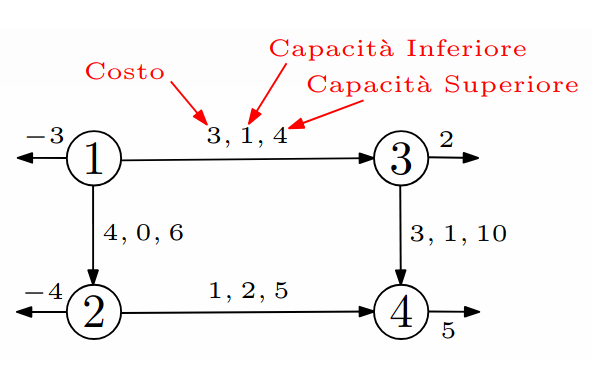
\includegraphics[width=0.6\textwidth]{img/esempio.png}
\end{figure}
\paragraph{Ipotesi semplificative: capacità inferiore nulla}
Per semplificare problema e notazione supponiamo che $l_{ij} = 0 \quad \forall (i,j)\in A$, e' sempre possibile farlo:
\begin{itemize}
  \item Data una rete $G$ esiste sempre una rete $H$ equivalente ad $G$ che abbia capacita' inferiori nulle.
  \begin{enumerate}
    \item si sottrae la quantita' $l_{ij}$ a $b_{ij}$ e a $u_ij$
    \item si aggiunge la quantia' $l_{ij}$ a $b_i$
    \item alla funziona obbiettivo bisognera' aggiungere
    \begin{align*}
      \sum_{(i,j) \in A} c_{ij}x_{ij}
    \end{align*}
  \end{enumerate}
  Ovvero al flusso $x_{ij}$ in $H$ corrisponde al flusso $x_{ij} + l_{ij}$ in $G$.
\end{itemize}
\paragraph{Ipotesi semplificativa: una sola sorgente e pozzo}
Spesso, nel progetto di algoritmi per problemi di flusso, conviene assumere che vi sia una sola sorgente e un solo pozzo.
\begin{itemize}
  \item Si può costruire una rete equivalente:
  \begin{itemize}
    \item Aggiungendo due nodi fittizi, uno corrispondente all’unica sorgente,
e l’altro all’unico pozzo.
    \item Aggiungendo archi fittizi dalla sorgente a ciascuna delle sorgenti
della rete di partenza. Tali archi avranno costo nullo, e capacità
superiore pari all’inverso dello sbilanciamento della sorgente.
    \item Aggiungendo archi fittizi da ciascuno dei pozzi della rete di partenza
al pozzo. Tali archi avranno anch’essi costo nullo, ma capacità
superiore pari allo sbilanciamento dell pozzo
  \item Lo sbilanciamento dell’unica sorgente sarà uguale alla somma degli
sbilanciamenti delle sorgenti. Similmente per il pozzo.
  \end{itemize}
\end{itemize}
\begin{figure}[H]
    \centering
    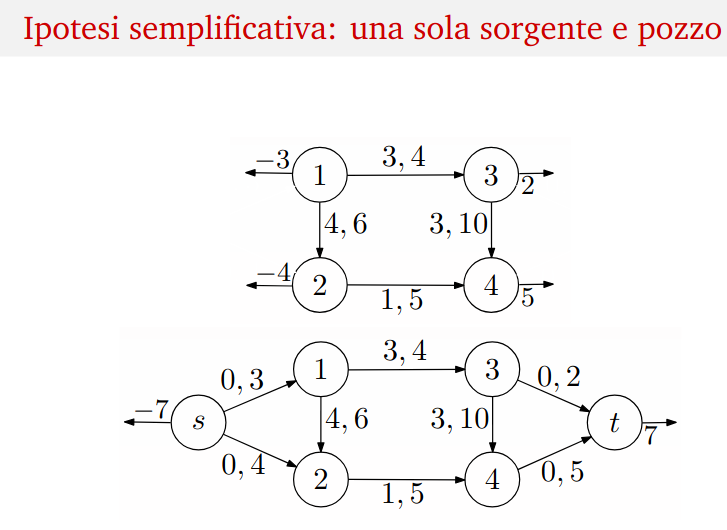
\includegraphics[width=0.6\textwidth]{img/singolopozzo.png}
\end{figure}
\paragraph{Capacità sui nodi}
Alcune volte è utile imporre che anche i nodi (e non solo gli archi) abbiamo delle capacita'
\begin{itemize}
  \item si sdoppia ogni nodo i con capacità in due nodi $i', i''$ in modo che:
  \begin{itemize}
    \item tutti gli archi entrati in $i$ entrano in $i'$
    \item tutti gli archi uscenti da $i$ partano da $i''$
    \item Si aggiunge un arco fittizio $(i', i'')$ con csoto nullo capacita' inferiore $l_i$ e capacita' superiore $u_i$
  \end{itemize}
  \begin{figure}[H]
    \centering
    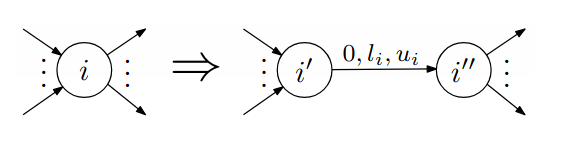
\includegraphics[width=0.6\textwidth]{img/capacitanodi.png}
\end{figure}
\end{itemize}
\subsubsection{Definizione e Modelli Matematici}
\paragraph{Problema del Flusso di Costo Minimo (MCF)}
\begin{align*}
  & \min cx \\
  & 0 \leq x \leq u \quad Ex = b
\end{align*}
con $c$ vettore costi, $u$ vettore capacita superiori, $E$ matrice di indidenza sui nodi e archi, $b$ vettore degli sbilanciamenti.\\
\vspace{2px}\\
Il \textbf{problema di flusso massimo} (o maximum flow, MF) è un
problema di ottimizzazione su reti che può essere visto come una
restrizione di MCF.\\
Ciò che cambia è la funzione obiettivo: non vogliamo minimizzare i
costi, ma piuttosto \textbf{massimizzare} i flussi.\\
\begin{align*}
  & \max v \\
  & \sum_{(j,s) \in BS(s)} x_{js} + v = \sum_{(s,j) \in FS(s)} x_{sj}\\
  & \sum_{(j,s) \in BS(i)} x_{ji} - \sum_{(i,j) \in FS(i)} x_{ij} = 0, \quad i \in N - \{s,t\}\\
  & \sum_{(j,s) \in BS(t)} x_{ji} = \sum_{(t,j) \in FS(t)} x_{tj} + v\\
  & 0 \leq x_{ij} \leq u_{ij}, \quad (i,j) \in A
\end{align*}
  \begin{figure}[H]
    \centering
    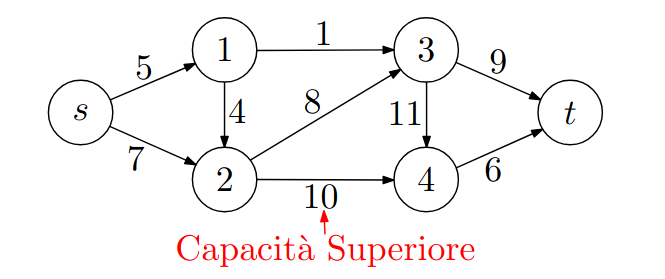
\includegraphics[width=0.5\textwidth]{img/max2.png}
\end{figure}
Il problema MF può essere visto come un caso particolare di MCF:
\begin{itemize}
  \item costi nulli
  \item sbilanciamenti nulli
  \item Si aggiunge però un arco fittizio da $t$ a $s$ con costo $-1$ e capacità infinita
\end{itemize}
  \begin{figure}[H]
    \centering
    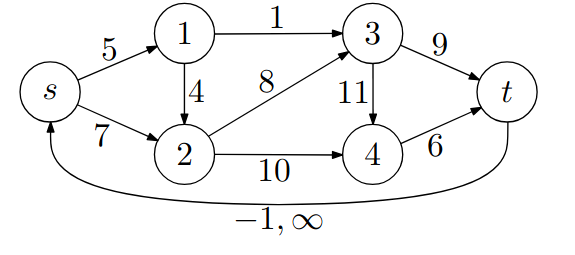
\includegraphics[width=0.5\textwidth]{img/fittizzio.png}
\end{figure}
\subsection{Il Problema del Flusso Massimo: Algortimi}
\fcolorbox{blue!75!black}{blue!5!white}{
\parbox{\linewidth}{
\textbf{Definizione}: Un taglio in una rete $G=(N,A)$ e' dato da una coppia $(N', N'')$ di sottoninsiemi di $N$ t.c. $N' \cap N'' = \emptyset$ e $N' \cup N'' = N$.\\
Un $(s,t)$-taglio in una rete $G$ e' un taglio $(N_s, N_t)$ dove $s \in N_s$ e $t \in N_t$.\\
\begin{itemize}
  \item Dato un $(s,t)$-taglio in $G=(N,A)$ indichiamo con $A^+(N_s, N_t)$ e $A^-(N_s, N_t)$ i seguenti sottoinsiemi di $A$:
  \begin{align*}
    & A^+(N_s, N_t) = \{(i,j) \in A | i \in N_s \land j \in N_t\} \\
    & A^-(N_s, N_t) = \{(i,j) \in A | i \in N_t \land j \in N_s\}
  \end{align*}
\end{itemize}
}}\\
\vspace{1px}\\
  \begin{figure}[H]
    \centering
    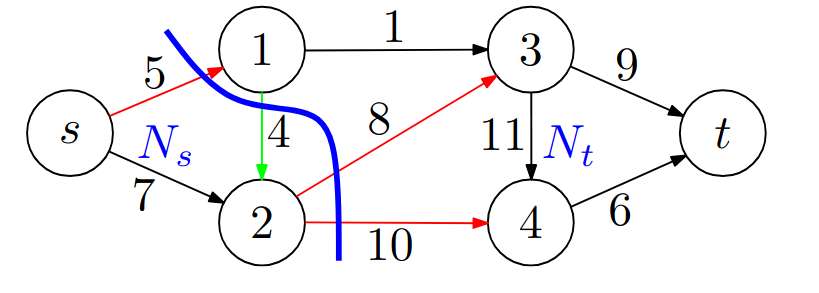
\includegraphics[width=0.5\textwidth]{img/taglio.png}
\end{figure}
\fcolorbox{blue!75!black}{blue!5!white}{
\parbox{\linewidth}{
\textbf{Lemma}: Per ogni $(s,t)$-taglio $(N_s, N_t)$ e ogni flusso ammissibile $x$ con valore $v$:
\begin{enumerate}
  \item \textbf{Flusso del taglio}: $v = \sum_{(i,j) \in A^+(N_s, N_t)} x_{ij} - \sum_{(i,j)\in A^- (N_s, N_t)} x_{ij}$; si indica con $x(N_s, N_t)$
  \item \textbf{Capacita' del taglio}: $v \leq \sum_{(i,j) \in A^+(N_s, N_t)} u_{ij}$; si indica con $u(N_s, N_t)$
\end{enumerate}
\begin{align*}
  v = x(N_s, N_t) \leq u(N_s, N_t)
\end{align*}
}}\\
\vspace{1px}\\
\paragraph{Cammini Aumentanti} Un cammino aumentante $P$ in una rete $G$ rispetto a $x$ non è nient’altro che un cammino semplice e orientato da $s$ a $t$ in $G_x$.\\
Dato un cammino aumentante $P$ rispetto a $x$, definiamo la capacità di $P$ rispetto a $x$ come:
\begin{align*}
  & \theta(P,x) = \min\{\min\{u_{ij} - x_{ij} | (i,j) \in P^+\}, \, \min\{x_{ij} | (j,i) \in P^-\}\}
\end{align*}
Dato un flusso $x$, un cammino $P$ in $G_x$ e un reale $\theta$, definiamo $x(P, \theta)$ il flusso definito come segue:
\begin{align*}
  (x(P, \theta)) = \begin{cases}
    x_{ij} + \theta & \text{ se $(i, j) \in P^+$}\\
    x_{ij} - \theta & \text{ se $(j, i) \in P^-$}\\
    x_{ij} & \text{ altrimenti}
  \end{cases}
\end{align*}
\subsubsection{Algoritmo di Ford-Fulkerson}
\fcolorbox{lime!75!black}{lime!5!white}{
\parbox{\linewidth}{
\begin{align*}
1. & x \gets 0\\[4pt]
2. & \text{Costruisci } G_x \text{ e determina se esiste un cammino aumentante } P.\\
        & \text{Se tale } P \text{ non esiste, termina e restituisci } x.\\[4pt]
3. & x \gets x(P, \theta(P,x))\\[4pt]
4. & \text{Ritorna al punto 2.}
\end{align*}
}}\\
\vspace{1px}\\
\fcolorbox{blue!75!black}{blue!5!white}{
\parbox{\linewidth}{
\textbf{Lemma}: Se $x$ e' ammissibile allora anche $x(P, \theta(P, x))$ e' ammissibile.
}}\\
\vspace{1px}\\
\fcolorbox{blue!75!black}{blue!5!white}{
\parbox{\linewidth}{
\textbf{Lemma}: Se $x$ e' un flesso ammissibile massimo, allora $G_x$ non ha cammini aumentanti.
}}\\
\vspace{1px}\\
\fcolorbox{blue!75!black}{blue!5!white}{
\parbox{\linewidth}{
\textbf{Lemma}: Se $G_x$ non ha camminni aumentanti, allora esiste un taglio di capacita' pari a $v$.
}}\\
\vspace{1px}\\
\fcolorbox{blue!75!black}{blue!5!white}{
\parbox{\linewidth}{
\textbf{Teorema (Correttezza)}: Se l'algoritmo di Ford-Fulkerson termina, allora il flusso $x$ è un flusso massimo.
}}\\
\vspace{1px}\\
\fcolorbox{blue!75!black}{blue!5!white}{
\parbox{\linewidth}{
\textbf{Teorema}: Il valore del amssimo flusso e' uguale alla minima capacita' dei tagli.
}}\\
\vspace{1px}\\
\fcolorbox{blue!75!black}{blue!5!white}{
\parbox{\linewidth}{
\textbf{Teorema}: Se le capacita' di $G$ sono numeri interi, allora esiste almeno un flusso intero massimo.
}}\\
\vspace{1px}\\
\subsubsection{Algortimo di Edmonds-Karp}
L’Algoritmo di Edmonds-Karp non è nient’altro che l’algoritmo di
Ford-Fulkerson dove, però, la ricerca del cammino aumentante
viene eseguita visitando in ampiezza (BFS) il grafo residuo $G_x$.\\
Notiamo che in questo modo i cammini aumentanti saranno
sempre cammini di \textbf{lunghezza minima}.\\
pagina 43

\subsubsection{Algortimo di Golberg-Tarjan}
\subsection{Il Problema del Flusso di Costo Minimo: Algoritmi}
\subsection{Problemi di Accoppiamento}

\fcolorbox{blue!75!black}{blue!5!white}{
\parbox{\linewidth}{
}}\\
\vspace{1px}\\




\section{Algoritmi per PL e PLI}
\subsection{Geometria Della Programmazione Lineare}
\begin{figure}[H]
    \centering
    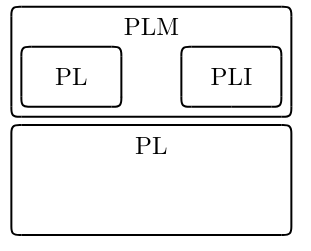
\includegraphics[width=0.3\textwidth]{img/PL.png}
\end{figure}
Lo spazio di ricerca, nei problemi PL, è in linea di principio infinito, però lo spazio di ricerca può essere in qualche caso ridotto ad un insieme finito, ossia l’insieme dei vertici del poliedro che definisce la regione ammissibile.\\
La domanda cui cercheremo di dare una risposta in questa prima sezione è la seguente: è possibile generalizzare quest’argomento al caso di problemi in $n > 2$ variabili?\\
\vspace{1px}\\
\fcolorbox{blue!75!black}{blue!5!white}{
\parbox{\linewidth}{
\textbf{Definizione Iperpiano}: Insieme $\{x \in \mathbb{R}^n | ax=b\}$ delle soluzioni dell’equazione lineare $ax=b$ dove $a \in \mathbb{R}^n$ e $b \in \mathbb{R}$
\begin{figure}[H]
    \centering
    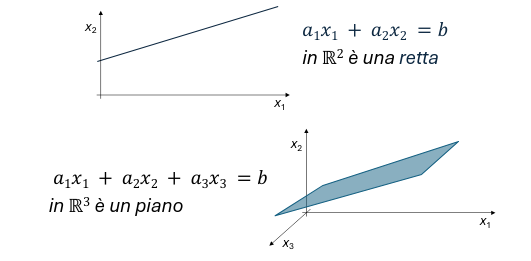
\includegraphics[width=0.5\textwidth]{img/iperpiano.png}
\end{figure}
}}\\
\vspace{1px}\\
\vspace{1px}
\fcolorbox{blue!75!black}{blue!5!white}{
\parbox{\linewidth}{
\textbf{Definizione Semispazio}: Insieme $\{x \in \mathbb{R}^n | ax\leq b\}$ delle soluzioni dell’equazione lineare $ax=b$ dove $a \in \mathbb{R}^n$ e $b \in \mathbb{R}$.\\
Un \textit{iperpiano} è il confine del corrispondente semispazio.
\begin{figure}[H]
    \centering
    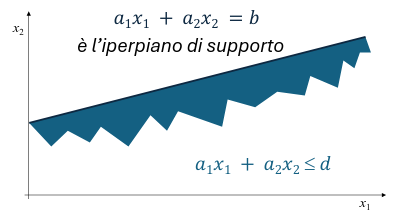
\includegraphics[width=0.5\textwidth]{img/semispazio.png}
\end{figure}
}}\\
\vspace{1px}\\
\fcolorbox{blue!75!black}{blue!5!white}{
\parbox{\linewidth}{
\textbf{Definizione Poliedro}: Intersezione $P$ di un numero finito $m$ di semispazi. Devono esistere una matrice $A \in \mathbb{R}^{m \times n}$ e un vettore $b \in \mathbb{R}$ tali che $P = \{x | Ax \leq b\}$.
\begin{figure}[H]
    \centering
    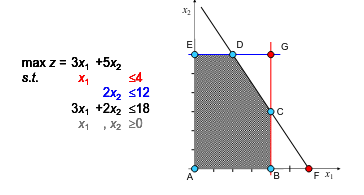
\includegraphics[width=0.5\textwidth]{img/poliedro.png}
\end{figure}
}}\\
\vspace{1px}\\
\fcolorbox{blue!75!black}{blue!5!white}{
\parbox{\linewidth}{
\textbf{Definizione Insieme convesso}: Un insieme $C \subseteq \mathbb{R}^n$ tale che tutti i punti che connettono $x, y \in C$ sono anche'essi in $C$ ossia
\begin{align*}
  \forall x, y \in C \quad \forall a \in [0,1] \quad ax+(1-a)y \in C
\end{align*}
\begin{figure}[H]
    \centering
    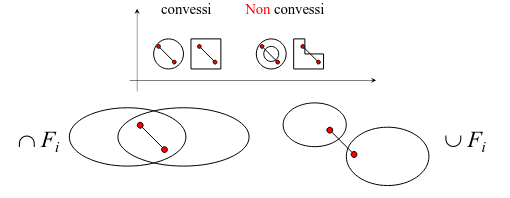
\includegraphics[width=0.6\textwidth]{img/convesso.png}
\end{figure}
}}\\
\vspace{1px}\\
\fcolorbox{blue!75!black}{blue!5!white}{
\parbox{\linewidth}{
\textbf{Definizione Faccia}: Se $I$ è tale che $P_I$ non è vuoto, chiamiamo il poliedro $P_I$ faccia di $P$.
}}\\
\begin{figure}[H]
    \centering
    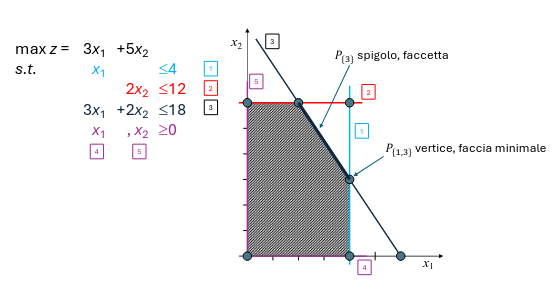
\includegraphics[width=0.7\textwidth]{img/facce.png}
\end{figure}
\paragraph{Soluzioni di Base}
Dato un poliedro $P=\{x | Ax \leq b\}$, supponiamo che $I=B$ sia t.c. $A_B$ matrice quadrata e invertibile. Allora:
\begin{itemize}
  \item $B$ e' detta base
  \item $A_B$ e' detta matrice di base
  \item $x_B = A_B^{-1}b_B$ e' detta soluzione di base
\end{itemize}
Una soluzione di base $x_B$ t.c. $x_B \in P$ e' detta \textbf{ammissibile}, altrimenti \textbf{non ammissibile}.\\
E' facile rendersi conto che i vertici di $P$ sono tutte e sole le sue soluzioni di base ammissibili.\\
\paragraph{Vincoli attivi}
Se $x\in P$ allora i vincoli che vengono soddisfatti come uguaglianze sono detti \textbf{attivi} in $x$. Indichiamo con $I(x)$ l'insieme degli indici dei vincoli attivi in $x$:
\begin{align*}
  I(x) = \{i | A_i x = b_i\}
\end{align*}
Per ogni $J \subseteq I(x)$ l'insieme $P_J$ e' una faccia di $P$, $P_{I(x)}$ e' la faccia minimale tra esse.\\
\fcolorbox{blue!75!black}{blue!5!white}{
\parbox{\linewidth}{
\textbf{Definizione Inviluppi Convessi}: I poliedri fin'ora li abbiamo rappresentati per facce, ma possono essere rappresentati anche per punti. \\
Dato un insieme di punti $X=\{x_1, \dots, x_S\} \subseteq \mathbb{R}^n$ \textbf{l'inviluppo convesso} di $X$ e' definito come l'insieme
\begin{align*}
  \text{conv}(X) = \{x = \sum_{i=1}^S \lambda_i x_i | \sum_{i=1}^S \lambda_i = 1 \land \lambda_i \geq 0\}
\end{align*}
Per esempio per $X=\{(1,3), (3,1),(2,5), (6,3)\}$
\begin{figure}[H]
    \centering
    
\includegraphics[width=0.4\textwidth]{img/conv.png}
\end{figure}
}}\\
\vspace{1px}\\
\fcolorbox{blue!75!black}{blue!5!white}{
\parbox{\linewidth}{
\textbf{Definizione Coni convessi}: Un insieme $C \subseteq \mathbb{R}^n$ e' detto \textbf{cono} sse per ogni $x \in C$ e pert ogni $a \in \mathbb{R}^+$ vale che $ax \in C$.\\
I coni che siano anche insiemi convessi (detti coni convessi) sono caratterizzabili equivalentemente come gli insiemi $C$ tali che
\begin{align*}
  x,y \in C \land \lambda, \mu \in \mathbb{R}^+ \Rightarrow \lambda x + \mu y \in C
\end{align*}
Anche per i coni convessi esiste una rappresentazione basata sulle direzioni: dato un insieme $V = \{v_1, \dots, v_t\} \subset \mathbb{R}^n$, il \textbf{cono finitamente generato} da $V$ è:
\begin{align*}
  \text{cono}(V) = \{v = \sum_{i=1}^t \mu_i v_i | \mu_i \in \mathbb{R}^+\}
\end{align*}
Per esempio per $X = \{(1, 3), (3, 1), (2, 5), (6, 3)\}$
\begin{figure}[H]
    \centering
    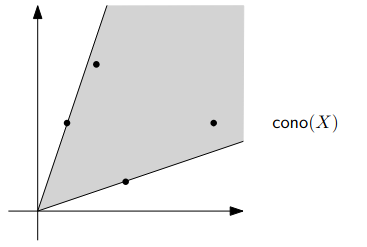
\includegraphics[width=0.4\textwidth]{img/cono.png}
\end{figure}
}}\\
\vspace{1px}\\
\fcolorbox{blue!75!black}{blue!5!white}{
\parbox{\linewidth}{
\textbf{Il Teorema di Motzkin (Decomposizione)} Dati $X, Y \subseteq \mathbb{R}^n$, indichiamo con $X + Y$ il sottoinsieme di $\mathbb{R}^n$ definito ponendo
\begin{align*}
  X + Y = \{x+y | x \in X \land y \in Y\}
\end{align*}
\textit{Teorema (Motzkin)}: $P \subseteq \mathbb{R}^n$ è un poliedro sse esistono $X, V$ finiti tali che $P = conv(X) + cono(V)$
\begin{figure}[H]
    \centering
    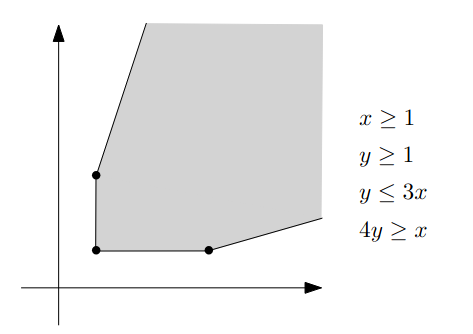
\includegraphics[width=0.4\textwidth]{img/Motzin.png}
\end{figure}
}}\\
\vspace{1px}\\
\paragraph{Due Rappresentazioni} 
\begin{itemize}
  \item Poliedri come intersezioni di semispazi
  \item Poliedri come somma di un politopo e di un cono
\end{itemize}
Le due rappresentazioni sono equivalenti (grazie al teorema di Motzkin) ma non hanno la stessa dimensione.\\
\vspace{1px}\\
\fcolorbox{blue!75!black}{blue!5!white}{
\parbox{\linewidth}{
\textbf{Teorema}: Sia $P = \{x | Ax \leq b\}$ e siano $x_1, \dots, x_s, v_1, \dots , v_t \in \mathbb{R}^n$ tali che
\begin{align*}
  P = \text{conv}(\{x_1, \dots, x_S\}) + \text{cono}(\{v_1, \dots, v_t\})
\end{align*}
Allora il problema $\max \{cx | Ax \leq b\}$ ha ottimo finito sse $cv_j \leq 0$ per ogni $j \in \{1, \dots , t\}$. In tal caso esiste inoltre un $k \in \{1, \dots , s\}$ tale che $x_k$ è una soluzione ottima.
}}
\subsection{Dualità, Direzioni Ammissibili e di Crescita}
La teoria della dualità è una branca dell’algebra lineare che risulta estremamente utile nella costruzione degli algoritmi per PL.\\
La teoria della dualità si basa sulla definizione di un’involuzione (ossia di una funzione inversa di sé stessa) che mappa ogni problema PL nel suo duale.
\begin{itemize}
  \item Primale: $\max \{cx | Ax\leq b\}$
  \item Duale: $\min \{yb | (yA=c) \land (y \geq 0)\}$
\end{itemize}
\paragraph{Proprietà Primale e Duale} È abbastanza facile dimostrare che il duale del duale è il primale.\\
\vspace{1px}\\
\vspace{1px}\\
\fcolorbox{blue!75!black}{blue!5!white}{
\parbox{\linewidth}{
\textbf{Teorema Debole di Dualità}: Se $\bar{x}$ e $\bar{y}$ sono soluzioni ammissibili per il primale e il duale, rispettivamente, allora $c \bar{x} \leq \bar{y} b$.\\
Corollario:
\begin{itemize}
  \item Se il primale è illimitato, allora il duale è impossibile (vuoto)
  \item Se $\bar{x}$ e $\bar{y}$ sono soluzioni ammissibili per il primale e il duale, rispettivamente, e $c \bar{x} = \bar{y} b$, allora $\bar{x}$ e $\bar{y}$ sono soluzioni ottime
\end{itemize}
}}
\paragraph{Direzioni Ammissibili — I} Data una coppia asimmetrica, consideriamento una soluzione ammissibile $\bar{x}$ per il primale, e chiediamoci se spostandoci lungo una direzione dell’iperspazio a partire da $\bar{x}$, si resta o meno nella regione ammissibile.\\
Un vettore $\xi \in \mathbb{R}^n$ e' detto \textbf{Direzione Ammissibile} se esiste $\bar{\lambda} > 0$ t.c. $x(\lambda) = \bar{x} + \lambda \xi$ e' ammissibile nel primale per ogni $\lambda \in [0, \bar{\lambda}]$.
\paragraph{Direzioni Ammissibili — II} Il vettore $\xi$ e' direzione ammissibile per $\bar{x}$ sse $A_{I(\bar{x})} \xi \leq 0$.
\paragraph{Direzioni di Crescita} Una direzione $\xi \in \mathbb{R}^n$ e' una \textbf{direzione di crescita} per $\bar{x}$ spostamento $\lambda$ lungo $\xi$ fa crescere il valore della funziona obiettivo ossia se:
\begin{align*}
  cs(\lambda) = c \bar{x} +\lambda c \xi > c \bar{x} \iff c \xi > 0
\end{align*}
La nozione di direzione di crescita, dunque, non dipende dal punto $\bar{x}$!
\subsection{L'algoritmo del Simplesso}
\begin{algorithm}[H]
\caption{Simplex Primal}
\begin{algorithmic}[1]
\State $N \leftarrow \{1,\ldots,m\} \setminus B$
\State $\bar{x} \leftarrow A_B^{-1} b_B$
\State $\bar{y}_B \leftarrow c_B A_B^{-1}$
\State $\bar{y}_N \leftarrow 0$
\If{$\bar{y}_B \ge 0$}
    \State \textbf{return} $\bar{x}, \bar{y}$ \Comment{soluzione ottima}
\EndIf
\State $h \leftarrow \min\{ i \in B \mid \bar{y}_i < 0 \}$
\State Sia $\xi$ la colonna di indice $h$ in $-(A_B^{-1})$
\If{$A_i \xi \le 0$ per ogni $i$}
    \State \textbf{return} $\xi$ \Comment{problema illimitato}
\EndIf
\State $k \leftarrow \arg\min \left\{ \frac{b_i - A_i \bar{x}}{A_i \xi} \mid A_i \xi > 0,\ i \in N \right\}$
\State $B \leftarrow (B \cup \{k\}) \setminus \{h\}$
\State \textbf{goto} 1
\end{algorithmic}
\end{algorithm}
L’algoritmo lavora mantenendo i seguenti tre invarianti:
\begin{itemize}
  \item $B$ e' una \textbf{base ammissibile}
  \item $\bar{x}$ e' \textbf{soluzione ammissibile} per il problema primale
  \begin{align*}
    \max \{cx | Ax \leq b\}
  \end{align*}
  mentre $\bar{y} A = c$.
  \item Di conseguenza, $\bar{y}$ è soluzione per il duale sse $\bar{y}_B > 0$
  \begin{align*}
    \max \{yb | yA = c, y \geq 0\}
  \end{align*} 
\end{itemize}
Se, quindi $\bar{y}B \geq 0$, allora l’algoritmo correttamente \textbf{termina}, restituendo $\bar{x}$ e $\bar{y}$ che sono soluzioni ottime per il primale e per il duale (riga 5.)\\
Se, invece, c’è un elemento di $\bar{y}$ strettamente negativo, allora non vale l’ottimalità. Cerchiamo quindi una direzione ammissibile e di crescita per $\bar{x}$.
\subsection{La tecnica Branch-and-Bound}
Finora ci siamo occupati della ricerca dell’ottimo in programmi lineari in cui tutte le variabili siano reali. Alla PLI si applica però una tecnica, detta branch-and-bound che, anche se esponenziale in tempo nel caso peggiore, permette in molti casi di evitare l’enumerazione esaustiva. \\
Perche' la tecnica del branch-and-bound sia applicabile ad una certa classe di problemi di ottimizzazione (che assumiamo di minimo), devono valere due requisiti:
\begin{itemize}
  \item \textbf{Rilassamento}: Deve essere possibile, in ogni momento, passare da un problema $\mathbb{P}$ ad un suo rilassamento $\mathbb{T} = \text{RELAX}(\mathbb{P})$, tipicamente più semplice da risolvere da un punto di vista computazionale. (In questo modo si possono facilmente calcolare limitazioni \textit{inferiori} al valore ottimo di $\mathbb{P}$.)
  \begin{align*}
    \text{RELAX}(\min \{cx | Ax \leq b \land x \in \mathbb{Z}^n\}) = \min\{cx | Ax \leq b\}
  \end{align*}
  \item \textbf{Branching}: Deve esistere un modo per \textit{partizionare} l’insieme delle soluzioni ammissibili di $\mathbb{P}$ ottenendo due sottoproblemi $\text{PARTITION}(\mathbb{P}) = (\mathbb{T}, \mathbb{Q})$.
  \begin{align*}
    \text{PARTITION}(\min\{cx | Ax \leq b \land x \in \mathbb{Z}^n\}) = \min \{cx | Ax \leq b \land x_i \geq n+1 \land x \in \mathbb{Z}^n\}
  \end{align*}
\end{itemize}
\begin{algorithm}[H]
\caption{Branch and Bound per $\mathcal{P}$}
\begin{algorithmic}[1]

\State $S \leftarrow \{\mathcal{P}\}$; \quad $v^* \leftarrow \infty$

\If{$S = \emptyset$}
    \State \Return soluzione ottima $x^*$ se definita
\EndIf

\State Scegli un problema $T \in S$; \quad $S \leftarrow S \setminus \{T\}$

\If{$\mathrm{RELAX}(T)$ è vuoto}
    \State \textbf{goto} 2
\EndIf

\If{$\mathrm{RELAX}(T)$ è illimitato}
    \State $(Q, S') \leftarrow \mathrm{PARTITION}(T)$
    \State $S \leftarrow S \cup \{Q, S'\}$
    \State \textbf{goto} 2
\EndIf

\State Siano $x$ e $v$ la soluzione e il valore ottimo di $\mathrm{RELAX}(T)$

\If{$v \ge v^*$}
    \State \textbf{goto} 2
\EndIf

\If{$x$ è ammissibile per $T$ \textbf{e} $v < v^*$}
    \State $v^* \leftarrow v$; \quad $x^* \leftarrow x$
    \State \textbf{goto} 2
\EndIf

\If{$x$ non è ammissibile per $T$ \textbf{e} $v < v^*$}
    \State $(Q, S') \leftarrow \mathrm{PARTITION}(T)$
    \State $S \leftarrow S \cup \{Q, S'\}$
    \State \textbf{goto} 2
\EndIf

\end{algorithmic}
\end{algorithm}
\end{document}
